\documentclass{chi2009}
\usepackage{times}
\usepackage{url}
\usepackage{graphics}
\usepackage{color}
\usepackage{wrapfig}
\usepackage[pdftex]{hyperref}
\hypersetup{%
pdftitle={Browsing the Web of Factual Claims},
pdfauthor={Beth Trushkowski and Rob Ennals},
pdfkeywords={CSCW, sensemaking, web, browsers, collaboration, mind mapping},
bookmarksnumbered,
pdfstartview={FitH},
colorlinks,
citecolor=black,
filecolor=black,
linkcolor=black,
urlcolor=black,
breaklinks=true,
}

\newcommand{\todo}[1]{}
% \newcommand{\todo}[1]{\footnote{{\bf TODO:} #1}}
\newcommand{\Intel}{Intel\textsuperscript{\textregistered}}

\newcommand{\idea}[1]{{\color{blue} IDEA: #1}\\}
\newcommand{\studyresult}[1]{{\color{red} STUDY RESULT?: #1}\\}
\newcommand{\howmany}{{\color{red} (HOW MANY?)}}

\pagenumbering{arabic}  % Arabic page numbers for submission.  Remove this line to eliminate page numbers for the camera ready copy


\begin{document}
% to make various LaTeX processors do the right thing with page size
\special{papersize=8.5in,11in}
\setlength{\paperheight}{11in}
\setlength{\paperwidth}{8.5in}
\setlength{\pdfpageheight}{\paperheight}
\setlength{\pdfpagewidth}{\paperwidth}
%
\toappear{Submitted for review to CHI 2009.}

\title{Browsing the Web of Factual Claims}

\numberofauthors{2}

\author{
	\alignauthor Authors anonymized for submission
}

%\author{
%\alignauthor Beth Trushkowsky\\
%       \affaddr{Computer Science Division}\\
%       \affaddr{University of California at Berkeley}\\
%       \email{trush@berkeley.edu}
%\alignauthor Rob Ennals\\
%       \affaddr{Intel Research}\\
%       \affaddr{2150 Shattuck Avenue}\\
%       \affaddr{Penthouse Suite}\\
%       \affaddr{Berkeley, CA 94704, USA}\\
%       \email{robert.ennals@intel.com}
%}

\sloppy 

\maketitle

\begin{abstract}

Conventional web browsing allows a user to look at pages and follow links between them; however when a user browses the web it is often not the pages themselves that they are looking for but  factual claims contained on those pages. A page may contain claims that are contradicted by other pages, or contain one interesting new claim hidden in a sea of claims that the user has already read. A user must thus invest significant effort extracting the claims that are accurate and interesting from the pages that they look at.

We present Think Link, a tool that overlays a web of factual claims on top of the web of pages. If a snippet of text on a web page makes a factual claim then a user can use Think Link to connect that snippet to other places on the web that make related claims. We argue that this makes it easier for users to determine the truth of claims made on the web.

\end{abstract}

\keywords{CSCW, sensemaking, web, browsers, collaboration, mind mapping} 

\category{H.5.2}{Information Interfaces and Presentation}{User Interfaces}[Graphical User Interfaces]

\section{Introduction}

The web provides users with a huge number of pages that they can read, but extracting useful and correct information from these pages can be difficult. Not everything on the web is true~\cite{bbcwebwarning}. If a user is to avoid incorrect factual claims then they will need to either stick to sources they can trust, or spend time looking for evidence on other web sites that supports or opposes what they have read. Similarly, a user will not find every claim on the web interesting. If a user is to locate claims that help them answer the questions they are interested in then they may have to spend considerable time reading claims that do not interest them in order to pick out those that do. Throughout this paper we will use the motivating example of a user who is worried about global warming and wants to find out what is going on and what they can do to help. Many web pages contain claims about global warming that are false, and many web pages repeat the same claims, making it difficult for a user to find interesting new facts that they were not previously aware of.

\begin{figure}[tb]
	\begin{center}
	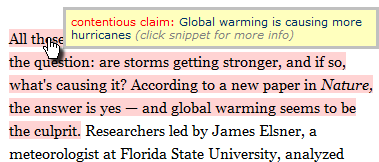
\includegraphics[width=6cm]{../screenshots/highlight_crop.png}
	\caption{Key factual claims are highlighted}
	\label{highlight}
	\end{center}
\end{figure}

\begin{figure}[tb]
	\begin{center}
	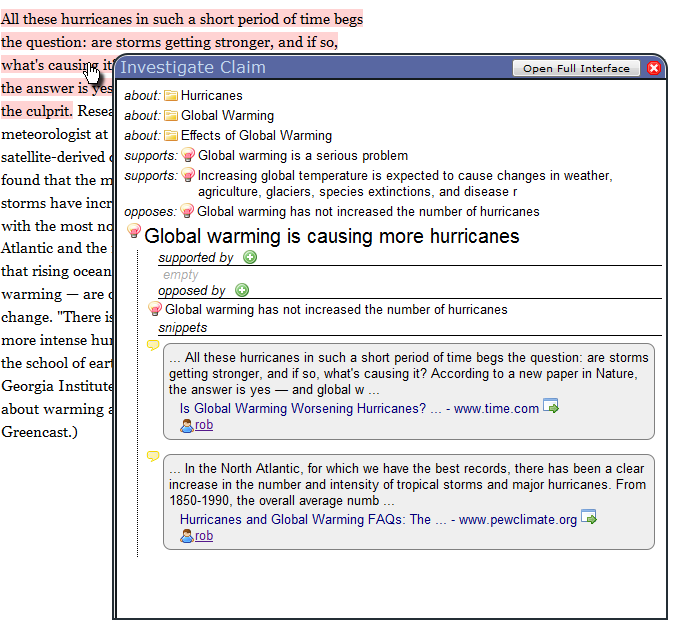
\includegraphics[width=8cm]{../screenshots/claim_popup_crop2.png}
	\caption{Click on a claim to investigate evidence for and against}
	\label{claimview}
	\end{center}
\end{figure}

The difficulty of finding correct information on the web has been discussed a lot recently. Tim Berners Lee has expressed concern about the difficulty that people face discerning whether information on the web is true~\cite{bbcwebwarning}. Many people have also voiced concerns about how easily people can subvert Wikipedia to give peolpe false information~\cite{wikifalse}. Several commentators have observed that there is a Media Echo Chamber effect~\cite{echochamber,echochamber2} in which news sources report claims that they have heard from other news sources, despite the fact that these claims may be misleading or untrue. If a user only reads news sources from a particular group then they may only be exposed to the views of that group and may not be aware that opposing views exist unless they actively seek them.  

Part of the problem is that conventional web browsing tools require the user to browse by looking at pages, when it is often not the pages themselves that the user is interested in but the factual claims contained within them. While a web page will typically contain links provided by the author of the page, these typically only reference a small proportion of the other pages that discuss the topic and are unlikely to include sources that disagree with the author. If the user wants to find all the 

 Moreover the best arguments supporting or opposing a claim may be distributed across a large number of disconnected pages, making it difficult for a user to assemble an argument from the pages on the web. The web is structured around where knowledge is coming from (pages written by particular authors) rather than what knowledge is about (the ideas contained on the pages). While this makes it easier for add knowledge to the web, it makes it harder for users to extract factual claims from it.



\begin{figure}[tb]
	\begin{center}
	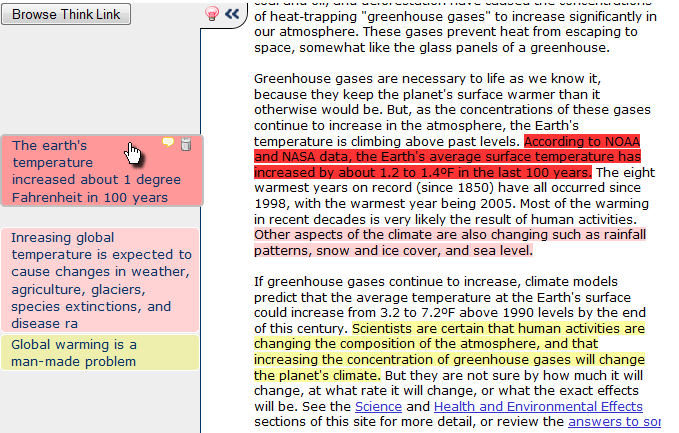
\includegraphics[width=6cm]{../screenshots/sidebar_crop.png}
	\caption{The margin summarizes the key claims on the page}
	\label{margin}
	\end{center}
\end{figure}



\subsection{Browse the Web of Factual Claims}

We have created a tool called Think Link that connects pages on the web to the factual claims being made on those pages, and allows a user to quickly find snippets of text on other web pages that make supporting or opposing claims. We hope that this tool will make it easier for users to identify incorrect claims in documents they read, and to quickly identify the best arguments for and against claims that they may be interested in.

As a user browses a web page Think Link will highlight snippets of text that make factual claims (Figure~\ref{highlight}). If a factual claim is contentious (meaning that other pages make opposing claims) then the highlight will be red. More information about highlighted claims can be found by either mousing over one of them, or opening the Think Link margin (Figure~\ref{margin}).

These highlighted claims serve as entry points to a browsable graph of factual claims. Clicking on a claim will pop up a window that allows one to easily view the other claims that support or oppose the selected claim, and the snippets of text on the web that make these claims (Figure~\ref{claimview}).

For example, if a user browsed a web page that claimed ``Global Warming does not exist'', then the text snippet that made this claim would be highlighted in red, indicating the fact that there are web pages elsewhere that make opposing claims. If the user were to click on the highlighted snippet then an ``investigate claim'' window would appear. This window would show that the claim ``Global Warming does not exist'' is opposed by the claim ``There is strong evidence for global warming''. If the user navigated to this new claim then they could quickly see the best claims that support the existence of global warming, and would be able to see summaries of the best sources that supported these claims.

\subsection{Collaborating to connect claims}

Think Link shares a lot in common with Wikis like Wikipedia~\cite{wikipedia}. The claim graph is shared between all users and editable by anyone. Any user can identify a claim made on a web page by selecting the web snippet that makes this claim and clicking the ``new snippet'' button on the browser toolbar. Similarly, any user can establish new supporting and opposing relationships between claims by using drag and drop within the claim browser. One can think of Think Link as being rather like a Wiki in which all the content is clipped from existing sources and links are created from those sources back to the wiki.

Think Link uses collaborative filtering~\cite{collective} to highlight the most interesting claims that support and oppose another claim, and the most interesting snippets that make a claim. If a user finds a snippet or claim interesting then they can mark it as such. When Think Link lists claims or snippets, it will show first those that the user marked as interesting, and order the rest according to the number of other users who marked them interesting.

\subsection{The Mental Model}

Think Link presents users with three kinds of object, each associated with a different family of icons (Figure~\ref{bookmark_icons}): 	

\begin{figure}[tb]
	\begin{center}
	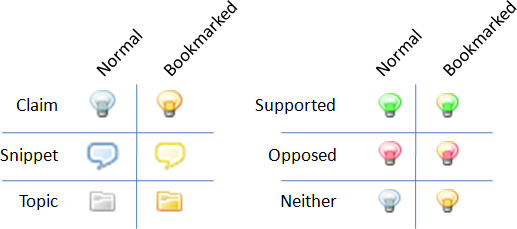
\includegraphics[width=8cm]{../screenshots/bookmark_icons.png}
	\caption{Icons used for Claims, Snippets, and Topics}
	\label{bookmark_icons}
	\end{center}
\end{figure}

%\begin{wrapfigure}{r}{4cm}
%	\begin{center}
%	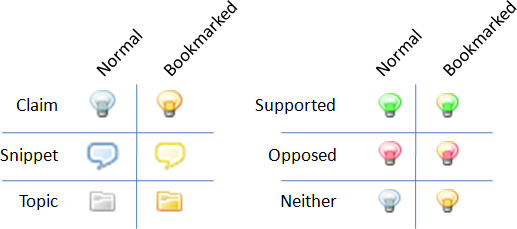
\includegraphics[width=4cm]{../screenshots/bookmark_icons.png}
%	\end{center}
%\end{wrapfigure}
\begin{itemize}
\item {\bf a claim} (
\includegraphics[width=0.3cm]{../images/lightbulb_off.png}) is a factual claim about the world that may be true or false. For example ``Global warming exists''. A claim may support or oppose other claims. Claims are written as raw English\footnote{though one can imagine supporting other languages in the future} text and are not understood logically by Think Link.
\item {\bf a snippet} (
\includegraphics[width=0.3cm]{../images/comment.png}) is a section of text on a particular web site that asserts or assumes the truth of a particular claim. Many snippets may assert the same claim and users are encouraged to re-use existing claims rather than creating new ones when creating new snippets.
\item {\bf a topic} (
\includegraphics[width=0.3cm]{../images/folder_grey.png}) is a thing that claims can be about. For example ``Global Warming'', or ``Computer Science''. A claim can have one or more topics that it is about, and a topic can have one or more more general topics. Topics are used both to organize, and to disambiguate claims. For example ``Bush'' can mean either ``George H W Bush'', ``George W Bush'', ``Vannevar Bush'', ``Kate Bush'', ``The Rock Band Bush'', or just ``A Bush''. Associating a claim with a topic allows one to write shorter claims without worrying about being ambiguous.
\end{itemize}

The three icons are used consistently when refering to these three object types. 
Yellow versions of these icons (
\includegraphics[width=0.3cm]{../images/lightbulb.png},
\includegraphics[width=0.3cm]{../images/folder.png},
\includegraphics[width=0.3cm]{../images/comment_yellow.png}) are used to identify claims, folders, or snippets that the user has marked as interesting.


\subsection{Why People Annotate}

Tools like Think Link rely on user contributions in order to be useful. If no users are identifying factual claims on pages then other people who browse such pages will not see any claims identified. Similarly, if no other users are connecting claims together, then users will not see any supporting or opposing claims when they click on a highlighted snippet.

Moreover, in order to become popular, a tool like Think Link needs to be useful even when very few people are using it. If a tool is only useful when it has a large community using it then it is unlikely that early adopters will stick with it enough for it to ever acquire a large community.

Our user study participants identified several reasons why they would want to mark up factual claims in documents they found. The most common reason people gave for identifying and organizing factual claims was if the person was writing an article or researching a topic and wanted to keep track of the information they had found. One user (who was an active blogger) also expressed an interest in finding and marking up instances of claims that he disagreed with, so that readers would see the arguments highlighted in red and be directed to the counter-arguments. The same user also expressed an interest in marking up claims in documents he had made in his own articles so that readers could quickly see the evidence he had found in support of his claims.

\studyresult{Quotes of users saying why they would use it}

\subsection{Contributions}

We believe that this work makes the following key contributions:

\begin{itemize}
\item We propose a new approach to browsing web pages that focusses on the factual claims made by these articles
\item We develop interaction techniques that make it easy for a user to browse the web through factual claims
\end{itemize}

\section{Interaction Techniques}

Users interact with Think Link in four key ways. Think Link will draw attention to interesting claims on pages that the user browses; it allows the user to identify new factual claims on pages they browse; it allows them to browse the graph of related claims and identify the strongest evidence supporting or opposing the claims they are looking at; and it allows them to organize the claim graph by making new connections between existing claims and topics.

\subsection{Exploring factual claims on a page}

When a user browses a web page, we want to make them aware of claims being made on the page that they might find interesting, or that other sources disagree with. Think Link draws attention to the factual claims that other users have identified on a web page by highlighting them (Figure~\ref{highlight}). Snippets are highlighted in red if they are contenious (other sources disagree with the claim), or yellow otherwise. The highlight colors are chosen such as to be pale enough to not impede reading, but dark enough to be noticeable. The colors are chosen to fit with people's normal associations with colors, where red is commonly associated with danger (e.g. a traffic light) and yellow is the standard color used for highlighter pens.

While a highlight lets the user know that a the snippet is making an interesting or contentious claim, the user may still wonder what claim the snippet has been identified as making. A snippet could be interpreted as asserting the truth of several claims. For example the phrase ``Alice and Bob live in Canada'' asserts both that Alice lives in Canada and that Bob lives in Canada. Similarly, a user may have eroneously marked a snippet as asserting a claim that it does not directly assert to be true. For example ``Alice and Bob live together''.

There are two ways that a user can identify the claims being made by the highlighted snippet; they can either hover their mose over a particular snippet to show information about that snippet (Figure~\ref{highlight}, or they can use the Think Link margin to show information about all snippets on the page (Figure~\ref{margin}).

The Think Link Margin is designed to mimick the traditional margin notes that readers often write on physical documents they are reading~\cite{marginalia}. A margin space is added to the left of the page containing a margin note for each snippet. Each margin note is aligned vertically with the claim it is about and contains the text of the claim. To emphasise the connection between a margin note and its associated snippet, a snippet is highlighted more strongly when the user mouses over the associated margin note (Figure~\ref{margin}). 

We found that when a participant sees a highlighted snippet, they will typically want to do one of four things: ignore it, remember it, delete it, or investigate it. If the user finds the snippet interesting and wants to use it later then they can bookmark it by clicking the bookmark icon that pops up when they mouse over the margin note. This will cause it to be displayed prominently in the claim browser (Section~\ref{claimbrowser}). If the user believes the snippet to not be making the claim that it says it does or otherwise badly marked up then they can delete the snippet by clicking on the trash can icon on the margin note. If the user thinks the claim is interesting and wants to see how it relates to claims made by other snippets on the web then they can click on either the highlighted text or the margin note to open the claim browser (Section~\ref{claimbrowser}).

A user can also use the margin to provide a quick overview of a document. They can scroll quickly through the document and look to see what key claims other users have marked in the margins. Several users remarked on how useful it was when reading a long document to be able to quickly scan through it and see what other users have thought were the most interesting points. \studyresult{put in some quotes}

\todo{sort out more consistent colors and icons between this view and the web view}
\todo{give the margin consistent colors with the highlight sections}
\todo{more nice zoomed-in screenshots showing the different interaction techniques}

\subsection{Browsing factual claims}
\label{browseclaim}\label{claimbrowser}

\begin{figure}[tb]
	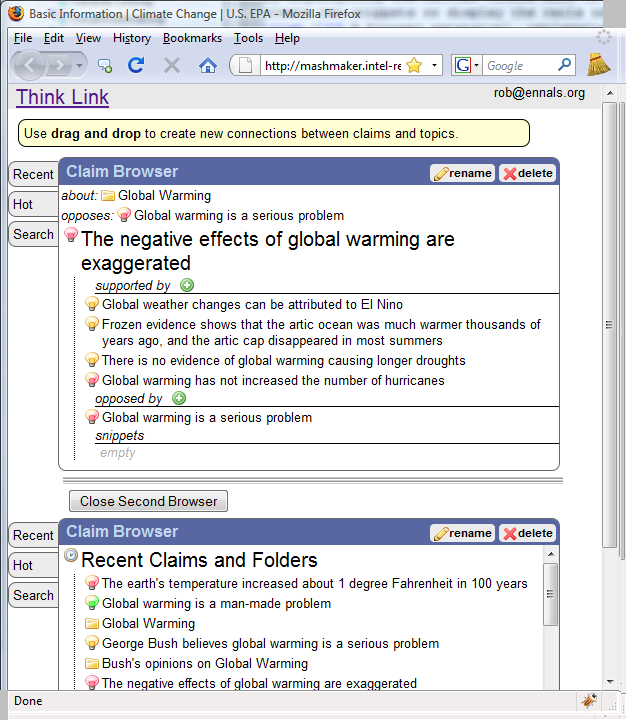
\includegraphics[width=8.5cm]{../screenshots/claimbrowse.png}
	\caption{The Claim Organizer contains two claim browsers}
	\label{fig:claimbrowser}
\end{figure}

\begin{figure}[tb]
	\begin{center}
	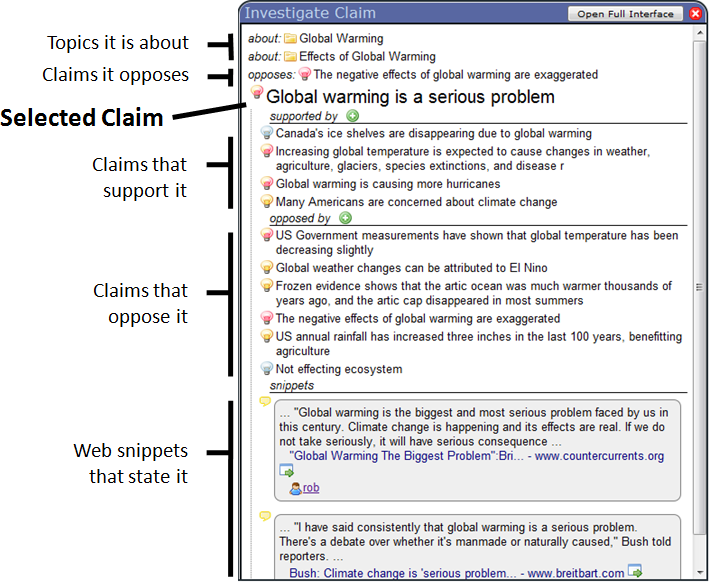
\includegraphics[width=8cm]{../screenshots/claimbrowse_diagram.png}
	\caption{The Claim Browser Allows one to browse the argument graph}
	\label{claimbrowse_diagram}
	\end{center}
\end{figure}

\begin{figure}[tb]
	\begin{center}
	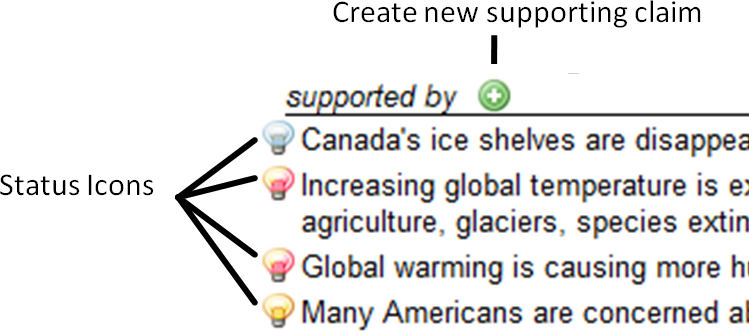
\includegraphics[width=8cm]{../screenshots/claimbrowse_zoom.png}
	\caption{Close up of a list of supporting claims}
	\label{claimbrowse_zoom}
	\end{center}
\end{figure}

\begin{figure}[tb]
	\begin{center}
	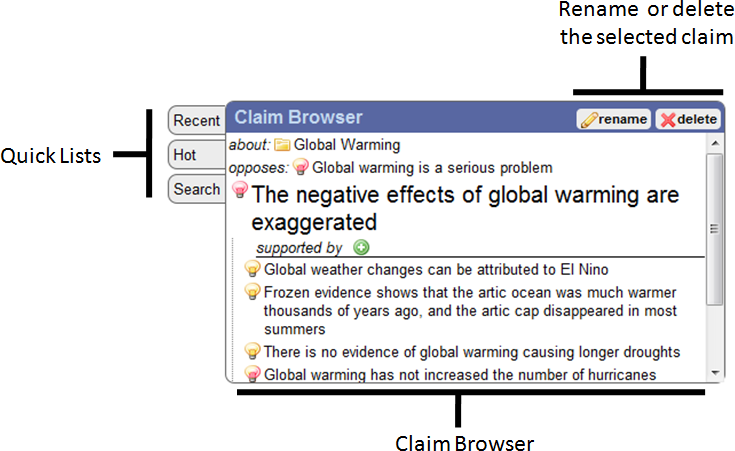
\includegraphics[width=8cm]{../screenshots/fullbrowser.png}
	\caption{The Enhanced claim browser adds additional controls}
	\label{enhancedbrowser}
	\end{center}
\end{figure}

Our users expressed an interest in using snippets to help them construct arguments that support a claim they agree with, to show them the arguments for and against a claim that they are unsure about, to collect evidence about a topic they are interested in, to share information with friends, and to see arguments against claims that they encountered on the web. We constructed the ``claim browser'' interface to help users do these things (Figure~\ref{fig:claimbrowser}).

Claims and topics form a directed graph structure. A claim can have any number of claims that support or oppose it, and any number of claims that it supports or opposes.
A topic can have any number of more specific topics (e.g. ``US Election 2008'' is more specific than ``US Elections'') and any number of more general topics. A topic can also have any number of claims about that topic.

When designing an interface to this structure, we were faced with two opposing constraints. We needed to be able to clearly view a large number of claims and topics in a small screen space, and we needed an interface that made it clear that the data was a graph rather than a tree. Dynamically reorganizing graphs such as those used in Vizster~\cite{vizster} and Personal Brain~\cite{thebrain} made the graph structure very clear, but made it difficult to clearly view large numbers of claims. Tree-based outliners such as OmniOutliner~\cite{outliner} made it easy to view large numbers of related claims, but made it difficult to present an impression of the data being a graph rather than a tree.

\todo{This interface is actually closer to TheBrain than the text suggests}

After several iterations, we settled on an interface that is a dynamically reorganizing graph layed out like an outliner. Like other dynamically reorganizing graphs, the interface is arranged around the currently selected node, and when a new node is selected the interface animates to surround the newly selected node with objects to relate to it. Like an outliner, the nodes that relate to the selected node are listed vertically below the selected node, each on their own line. Our users commented that they found it quite intuitive to navigate through a graph of claims and topics in this way. \studyresult{quote}.

The placement of objects above and below is intended to emphasize the conventional structuring of an argument graph (Section~\ref{argumentgraph}), with topics going upwards and arguments for and against a claim going downwards. A user can navigate down to get to explore why a claim may or may not be true, or navigate up to find out about more general topics, or claims that the selected claim supports or opposes.

\todo{Have I seen an interface like this elsewhere? Did PARC have something like this?}

\todo{Is this interface a contribution in itself? Has an interface like this been presented before?}

Animation is used throughout the interface to give users a sense of where they are and how the current interface state related to previous states. When a new item is selected, it grows in size and moves to the center. Other items that were already on the screen move from their current locations to their new locations. Other objects appear and disapper by smoothly sliding into or out of view. We found that this animation helps users retain a sense of where they are with respect to what they were looking at previously and helps users avoid getting lost (Section~\ref{gettinglost}).

Users see a claim browser in three different places:
\begin{itemize}
\item {\bf The Main Organizer} shows two claim browsers, and allows users to use drag and drop to make new connections between claims in the two organizers. (Figure~\ref{fig:claimbrowser})
\item {\bf The Popup Browser} shows one claim browser in a reduced-size window and is used to quickly investigate a claim found on a web page. (Figure~\ref{claimview})
\item {\bf The Claim Selection Window} shows one claim browser, together with the text of a new snippet, and is used to identify the claim that a snippet is making. (Figure~\ref{snipsavecrop}) 
\end{itemize}


\subsection{Identifying new factual claims}
\label{newsnippet}

\begin{figure*}[tb]
	\begin{center}
	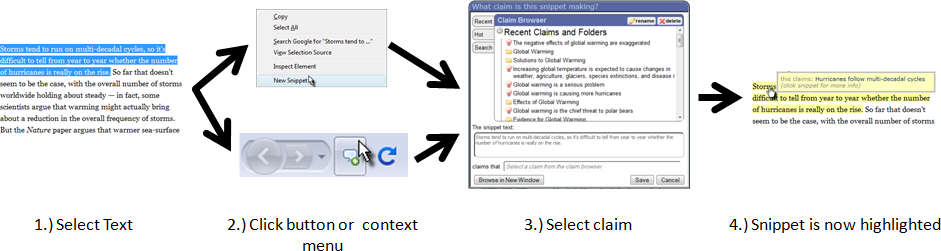
\includegraphics[width=16cm]{../screenshots/newsnip_all.png}
	\caption{Process for creating a new snippet}
	\label{createprocess}
	\end{center}
\end{figure*}

%\begin{figure}[tb]
%	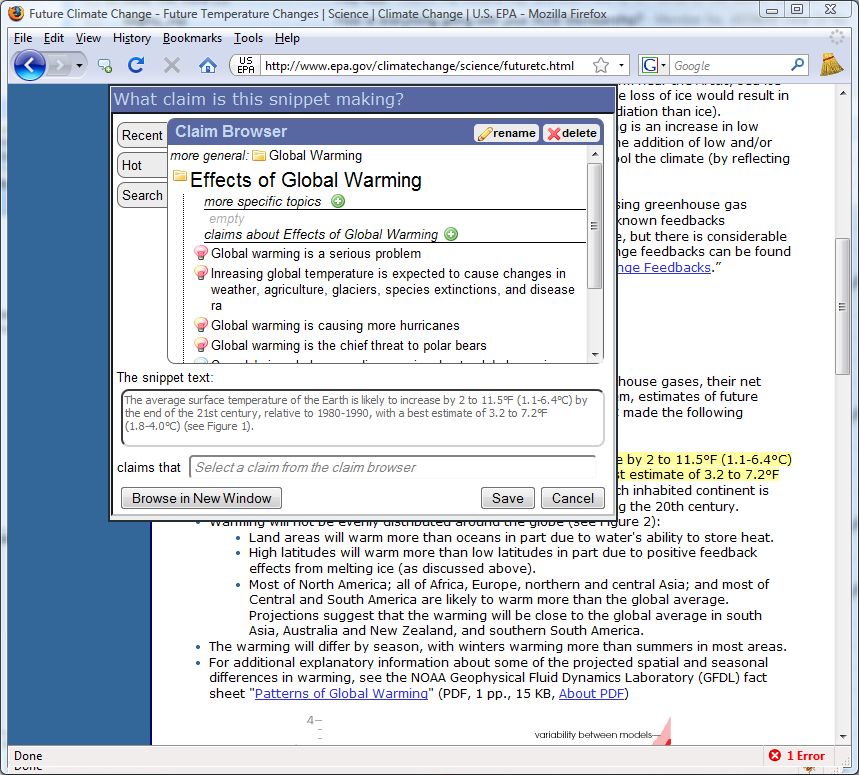
\includegraphics[width=8.5cm]{../screenshots/snipsave_full.png}
%	\caption{The claim selection window allows one to identify the claim a snippet is making}
%	\label{snipsavefull}
%\end{figure}

\begin{figure}[tb]
	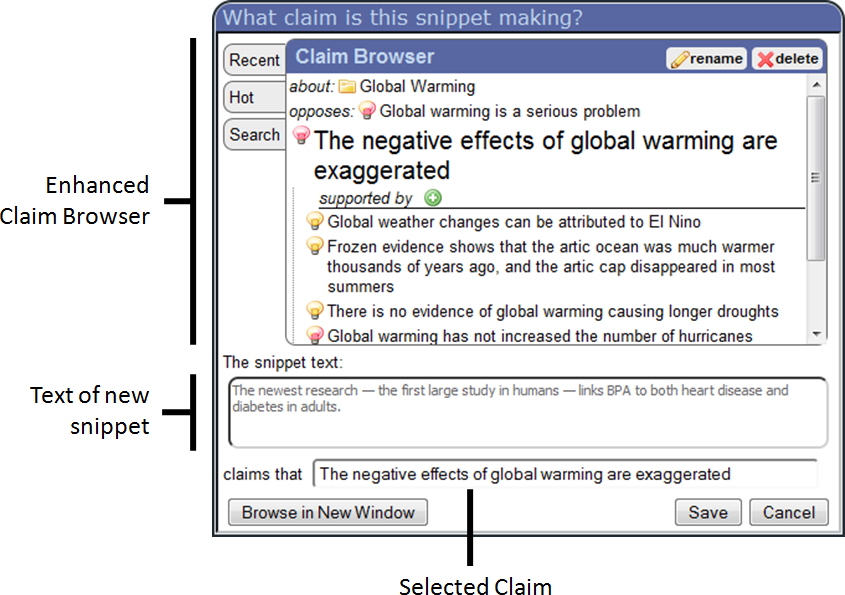
\includegraphics[width=8.5cm]{../screenshots/snipsave_diagram.png}
	\caption{Selecting the claim made by a new snippet}
	\label{snipsavecrop}
\end{figure}


If a user finds a snippet of text on a page that makes an interesting claim then they may want to enter it into Think Link. There are several reasons they may wish to do this. It may be that they find the snippet useful and may want to refer to it again in the future. It may be that they disagree with the claim, and want to alert other readers to the fact that there are opposing arguments, or it may be that they agree with the claim and want to provide easy access to evidence that backs it up. 

To create a new snippet, the user selects the text to be included and then either clicks on the ``new snippet'' button on the browser toolbar, or selects the ``new snippet'' option from the context menu that appears when they click the right mouse button. This is a similar approach to that taken clipping tools such as Google Notebook~\cite{googlenotebook}.

Once the user has identified the text in a snippet, they need to identify the claim that the snippet is making. To do this, Think Link presents the user with a ``claim selection'' window. This window contains a small version of the claim browser (Section~\ref{browseclaim}) that the user can use to select the claim that the snippet is making. At the bottom of the window, we show the phrase ``the snippet text {\it snippet} claims that {\it claim}''. We found that this helps users understand the nature of a claim and its relationship to a snippet (Section~\ref{study-claimmeaning}).

Since much of Think Link's utility comes from linking snippets together, it is important that to encourage users to reuse existing claims rather than creating new ones, and that when users do create new claims they connect them to existing claims and existing topics. Motivated by this, we designed the claim selection window to make it easier to pick out an existing claim than to create a new one. Moreover, one cannot create a new claim without connecting it to an existing topic or an existing claim. To create a new claim, one navigates to a topic that the claim is about, or a claim that the new claim supports or opposes, and then clicks on the (
\includegraphics[width=0.3cm]{../images/add.png}) button on the list that one wishes to add the new claim to. For example, if the new claim opposes an existing claim, then one clicks the (
\includegraphics[width=0.3cm]{../images/add.png}) button on the ``opposed by'' heading for the existing claim.

This is an intentionally different model to that used by ad-hoc tag-based~\cite{tags} systems such as Delicious~\cite{delicious} and Flickr~\cite{flickr}. This is because in bookmarking or image storing systems it is not so important that duplicates be avoided and that objects be well connected.

In earlier revisions of the interface it was very easy for users to quickly create new claim texts and awkward to find and reuse existing ones. This led users to create many claims that were essentially equivalent and reduced the utility of Think Link as a tool for connection snippets together (Section~\ref{study-reuse}). 

\todo{Make new snippet icon throb when something is selected}



\subsection{Organizing factual claims}

Much of the value of Think Link comes from the connections between claims. It is thus important that it be easy to establish new connections between claims and topics. 

Think Link uses the familiar drag and drop interface for establishing new connections. To establish a connection between two claims, one need simply drag one claim onto the other. In the full interface, one can open two browsers and drag points from one browser onto points on the other.

In our initial study, we found that many users did not realize that they could use drag and drop to create connections to existing claims. We rectify this, we added a notice at the top of the main organizer window (Figure~\ref{fig:claimbrowser}) telling users that they can use drag and drop.

We found that creating new connections between existing claims was one of the things that users found most difficult.

\todo{say more here}

\section{Discussion}

\subsection{Context of a Claim}

\subsection{How many claims to show}

\subsection{Beyond Claims}

\section{Implementation}

Think Link is implemented as three largely independent components:

\begin{itemize}
\item {\bf A server}, written using Ruby, PHP, and MySQL that maintains a graph of claims, topics, and snippets and provides an API that allows this data to be queried and modified
\item {\bf A web UI}, written using Ruby on Rails~\cite{rails} that provides a visual interface to the claim graph
\item {\bf A page enhancement script}, written in Javascript, that augments the page it is run on by highlighting the factual claims made on the page. This script also provides the ability to create new snippets or display the rails interface to investigate a particular claim.
\item {\bf A browser extension}, implemented for Firefox~\cite{firefoxextension}, that inserts the page enhancement script into all pages the user browses to, and provides toolbar and context-menu shortcuts to the ``new snippet'' feature of the page enhancement script.
\end{itemize}

These components are largely independent. One could use the javascript script on a web page without using the firefox extension, by either manually including it on the page (e.g. to enhance your own blog) or by adding it using a proxy. Since the server API is public, one could write alternative tools that mark up web pages in different ways, or use the claim graph for different purposes.

The source code to Think Link is publicly available under the Apache license at the following URL:

{\b url removed for blind submission}

We expect to have a public deployment available by the time of publication.

We use icons from the free FamFamFam Silk~\cite{silkicons} collection.



\section{Investigative Study}

We performed two ``think aloud'' studies to guide and evaluate the development of Think Link. The aim of the first study was to see how users normally browse the web and to see how they might try to use an initial prototype of Think Link to help them. 

We recruited 12 paid participants. Five were female, seven were male. Their ages ranged from high school age to retired. Our intention was to recruit users who were not experts, but who regularly used the internet to find information. We recruited participants using a posting to the Craigslist~\cite{craigslist} classified adverts site. In our advert, we expressed an interest in people who use the internet to gather knowledge, rather than just for tasks such as email or shopping. We filtered participants based on their short answers to questions about how they found, organized, and shared information on the web. 

\subsection{Protocol for the First Study}

Study sessions took approximately 45 minutes. Participants were seated at a single-screen workstation with the Firefox browser, augmented with the Think Link plugin. We first demonstrated Think Link's interface, and then asked them to perform two tasks. In the first task, we asked them to use Think Link to gather information about a political topic that was of interest to them and currently in the news. For the second task, we asked them to browse the web in a way that would typically do so at home or at work, and see if they could use Think Link to help them do so.

In the second task, we wanted to leave users relatively unconstrained so that we could see how users might try to use a tool like this during their normal browsing, rather than how well they could accomplish a pre-set task that they might never attempt in normal life. For the first task, we constrained the task to an a topic for which we had already marked up a number of claims, to increase the likelyhood that users would encounter existing claims.

The focus of this study was on whether people would be able to gather snippets on the web and structure them into a coherent argument graph, rather than on how they would react when they browsed to a page where an argument had already been identified - which was one of the focusses of our second study.

In this initial study, users were exposed to the prototype interface shown in Figures~\ref{oldsnippetbox} and \ref{oldbrowser}, rather than the final interface described in Section~\ref{interface}.

\subsection{Findings}

All the participants were able to create new snippets. Participants had little difficulty identifying interesting claims being made by web pages, selecting appropriate sections of text, and either picking existing claims that were appropriate, or writing appropriate new claims. Most ($9/12$) stated that they found it easy to create new snippets and associate them with claims.
In the initial interface snippets were only highlighted when the margin was open. This confused some participants ($5/12$) who were surprised to not see their snippets highlighted when they created them. In the final interface, we addressed this problem by always highlighting snippets.

In the initial interface the button to open the margin was on the toolbar, next to the ``new snippet'' button. This led some participants ($4/12$) to get confused about which they should use in each case. In the final interface, we addressed this problem by putting the margin button on the side of the page, with a chevron to indicate that it will pull out a margin (Figure~\ref{marginpull}).

\begin{figure}[ht]
	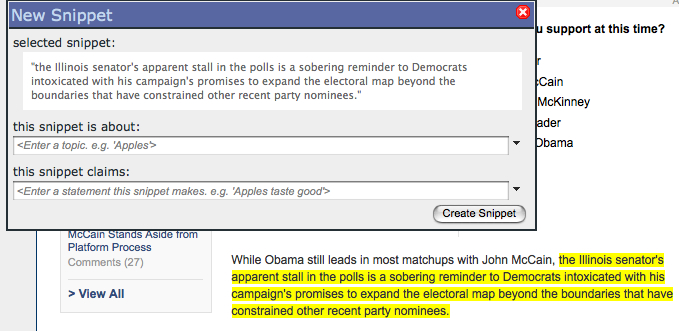
\includegraphics[width=8.5cm]{../screenshots/snippetdialog_sm.jpg}
	\caption{First Prototype Snippet Creation Dialog}
	\label{oldsnippetbox}
\end{figure}

In the initial interface we used a simplified snippet creation window (Figure~\ref{oldsnippetbox}) that was intended to make the process of snippet creation very lightweight. This window contained two text boxes. The first of these boxes was for the topic (e.g. ``Global Warming'') and the second of the boxes was for the claim (e.g. ``Global Warming is Man Made''). Both of these boxes used an auto-complete drop-down list to suggest appropriate existing topics or snippets as the user typed, 
biasing towards topics that were recent or hot. 

Most ($7/12$) users got confused between topics and claims at some point, either entering a topic as a claim, or entering a claim as a topic. We felt that this was partly because the snippet creation interface (Figure~\ref{oldsnippetbox}) gave the user little impression of how their snippet would appear in the claim browser. In the final interface we addressed this problem by giving the snippet creation interface the same core UI as the claim browser interface (Section~\ref{newsnippet}). We also decided to change our name for a factual claim from ``point'' to ``claim''.

While most ($10/12$) reused a topic that they had created or someone else had created, many ($6/12$) had a tendency to ignore the suggestion box and type new claims rather than looking for existing claims that might be a good match for their snippet. For the final interface, we tried to encourage users to reuse existing claims rather than writing new ones by making it easier to browse existing claims from the snippet creation window, and requiring users to click a 
\includegraphics[width=0.3cm]{../images/add.png} button in order to create a new claim (Section~\ref{newsnippet}). 

Our initial interface for claim browsing (Figure~\ref{oldbrowser}) caused several ($5/12$) to remark that they felt they were confused about where they were in the claim graph. This interface had a separate page for each claim or topic, rather than animating between them, making it easy to lose track of ones position in the graph of points. Several ($2/12$) remarked that part of the problem was that it wasn't obvious that the various boxes on the page were information about the claim in large text. For the final interface we addressed this problem by using animation to maintain a sense of where things were when the focus changed, and by placing information about a point around that point rather than in separate boxes (Section~\ref{claimbrowser}).

All users had some difficulty connecting existing claims together. The first four participants were a different interface in which new connections were made by clicking on an ``add'' button, and then typing the name of the claim into an auto-complete box. Users found this approach difficult as it required them to remember the text of claims that they had seen recently. In light of this, after the first four participants we switched to a drag and drop interface (Figure~\ref{oldbrowser}).

The drag and drop interface worked better. Most ($7/8$) users were eventually able to use the new interface proficiently. However all users initially found the drag and drop interface confusing, and no users guessed that they could connect existing points using drag and drop. We identified this as an area needing improvement in the next interface revision.


\begin{figure}[ht]
	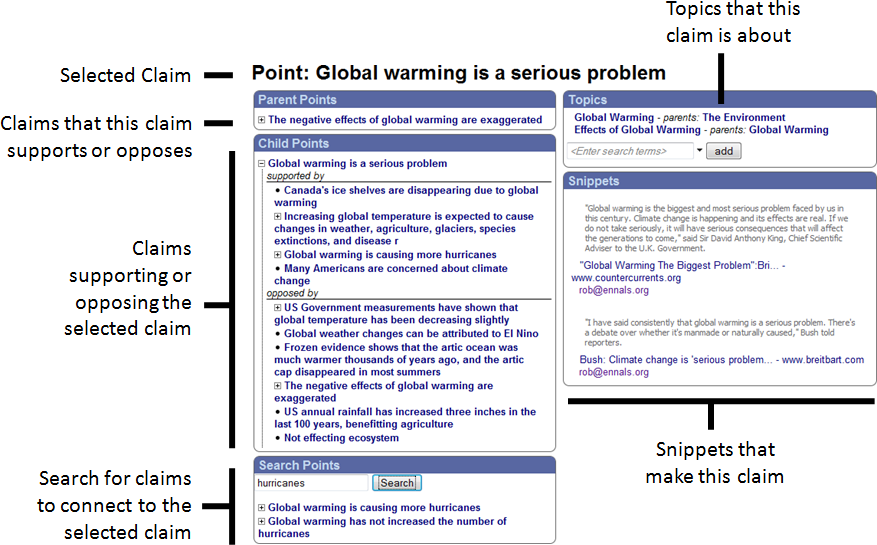
\includegraphics[width=8.5cm]{../screenshots/oldpoint_diagram.png}
	\caption{Initial Prototype Claim Browser}
	\label{oldbrowser}
\end{figure}

Many ($7/12$) participants also expressed a desire to organize claims into connected arguments during their session. Of these seven, we noticed that four would alternate between creating new snippets and organizing their claims in the claim browser (Section~\ref{claimbrowser}). With each new claim, users would create relationships between existing claims.

Many ($6/12$) participants marked one claim as supporting another claim when in fact they should have both been marked as supporting a shared claim that needed to be created. For the final interface we tried to address this problem by making the graph structure of claims easier to visualize and making it easier to create new claims (Section~\ref{claimbrowser}).

Two participants wanted to mark up a table as being a snippet and were unsure what claim they should say it made. In both cases, the table was a table of gold medals from the Beijing Olympics. We identified this as an area that we should investigate adding support for, since a table can provide evidence for the truth of many interesting claims.

One participant falsely connected claims that were actually referring to similar events that took place at different times rather than really being the same event. We identified the need for Think Link to provide more support for identifying the point in time that a claim or snippet is discussing.

Most ($9/12$) stated that they found the tool easy to use, and many ($5/12$) expressed an interest in using it during their normal browsing in its current state. When asked what they would want to use Think Link for, the most popular uses were helping them write a document ($5/12$), helping them form a personal opinion ($5/12$), or helping them argue a point to others ($5/12$). Many ($5/12$) were interested in seeing claims and snippets identified by their friends. Two said they were not interested in seeing what other people thought was interesting. Three users expressed an interest in using Think Link in ways that do not fit well with the current design, including gathering information about products they might buy, or finding cheap flights.

Due to the nature of the task, few ($3/12$) participants browsed pages that contained claims highlighted by other people, and so we were not able to evaluate how people reacted to seeing such highlights. This was made a priority of the second study.

\todo{mention people not being sure how broad a topic should be}
\todo{mention people creating claim in one topic and not being found in other related topics}


\section{Evaluation Study}

The purpose of the second study was to evaluate whether the interface changes we had made in reaction to the first study had made the tool usable. 

We recruited 6 paid participants. Four were female and two were male. Although we recruited participants using the same advert as the first study, the timing of our second advert around the beginning of the semester meant that five of the participants were students. Since the second group was different demographically to the first group, it is not possible to make a direct comparison between their behaviours. However we were still able to make interesting observations about how users used the new interface.

\subsection{Study Protocol}

In the second study we were more confident about the usability of our tool and so we decided to tell them nothing about how to use it. We gave each user a brief introduction to the aims of the tool, and then asked them to perform two tasks with it. The first task was to look at a selection of web pages that already had highlights and tell them to explore the interface. The second task was to identify claims on a page that had not been marked up and connect them appropriately to existing claims.

Unlike the first study, we specified the pages that our users should look at. This was because we wanted to see how users would react to seeing pages in which core claims had been marked up as snippets, and wanted to be sure that new snippets people identified had related claims in our database.

Participants were shown an interface that is largely identical to that described in Section~\ref{interface}. All changes are described in the text below.

\subsection{Findings}

All the participants were very enthusiastic about the new interface. Most \howmany participants expressed a strong interest in being able to use the tool now. One user commented ``I can see myself getting quite addicted to this''.

When shown a page with highlighted text, all users noticed that text had been highlighted and all users were able to infer that red highlight meant that the point was contentious. All users worked out that they could get more information about a claim by clicking on it. Most \howmany users did not immediately notice the presence of the margin button or the fact that Think Link had a margin feature, suggesting that the icon may need to be animated or perhaps made bigger.

Several \howmany users were very enthusiastic about the ability to see when other users thought a claim on a page was contentious, and the ability to quickly navigate to contradictory arguments. One user commented ``The web needs to be taken with a grain of salt, and this gives you salt goggles''.

The problems we had identified with the prototype interface seemed to have been fixed --- though, given the different demographics, we cannot state this conclusively. Everybody found it easy to tell what the ``open margin'' and ``new snippet'' buttons did. Nobody got confused between topics and claims. 

Users seemed to enjoy the process of browsing through the graph of claims, seeing what supporting and opposing arguments had been identified, and what snippets had been found about topics.

Many ($4/6$) wanted to have a ``back'' button to help them navigate through the claim graph, but all users were comfortable navigating backwards once they noticed that the place they had come from was shown as a link at the top of the display.

Most users \howmany still seemed to find the process of creating connections between existing claims confusing, at least at first. Several \howmany users tried to create a connection to an existing point by clicking on the 
\includegraphics[width=0.3cm]{../images/add.png} button, rather than by dragging the existing point over. This prompted us to display a message in this case (Figure~\ref{newdragmessage}). Most \howmany users did not not immediately realize that they could use drag and drop. This prompted us to add a prominent message at the top of the claim browser encouraging users to use drag and drop to organize claims and points. All users were able to successfully organize points and claims with drag and drop once they had realized that this is what they were supposed to do.

Many users \howmany uncovered a bug in our new snippet window. They would navigate to an existing claim and then click the 
\includegraphics[width=0.3cm]{../images/add.png} button to create a new supporting or opposing claim. However they would then click ``Save'' before they had pressed return to create the new claim, with the result that their new snippet was attached to the selected claim rather than the new claim. This bug was easily fixed...

One user said they wanted to be able to mark a claim on a web page as being wrong without having to find other snippets that argued against it. In future work we plan to offer such a feature by allowing users to say whether they believe a claim is true.

\todo{quote collection}

\section{Related Work}

Think Link is influenced by previous work in a number of fields. Most notably, the idea of a collectively edited space in which people can create shared descriptions of topics is influenced by Wikis, the dynamic graph interface is influenced by mind mapping tools, the structuring of arguments as a graph is influenced by argumentation graphs, and the approach to gathering snippets from web pages is influenced by existing web clipping tools.

\subsection{Wikis}

Wikis like Wikipedia~\cite{wikipedia} allow many authors to collaborate together to build a single shared document about a topic. Wikis thus achieve Think Links's goal of putting all information about a particular factual claim in one place, rather than scattering knowledge across a number of pages, each authored by a different writer. Indeed one can Think of Think Link as being a bit like a wiki in which all content is transcluded~\cite{transclusion} from existing sources and implicit links are added back from those sources to the wiki page to allow readers of other pages to easily see how they relate to arguments elsewhere.

Wikipedia's greatest strength is also its greatest weakness. Since anyone can edit Wikipedia, there is always the danger that the information one reads could be incorrect~\cite{wikifalse}. Several projects have attempted to address this problem by tracking sources of edits~\cite{wikicorrect}, but it is difficult to remove the problem entirely. While Think Link also allows anyone to edit its argument graph, all snippets come from known sources, making it easier to see where claims have come from and whether trustworthy sources agree with them.

\subsection{Web Clipping and Annotation Systems}

Web clipping tools such as Google Notebook~\cite{googlenotebook}, Scrapbook~\cite{scrapbook}, and Zotero~\cite{zotero} allow one to gather and organize interesting from web pages. Several of Several of these tools also allow one to share one's collection of snippets with other people that one may be collaborating with. 

Many web clipping systems are also web annotation systems. Web annotation systems such as ShiftSpace~\cite{shiftspace}, Stickis~\cite{stickis}, DrawHere~\cite{drawhere}, SharedCopy~\cite{sharedcopy}, and Diigo~\cite{diigo} allow people to add annotations to existing web pages and view annotations written by other people. Common annotations include commenting on perceived inaccuracies, highlighting interesting passages, or linking to other relavent documents. More generally, tools like WBI~\cite{personalweb} and Mash Maker~\cite{mashmaker} allow arbitrary changes to be made to web pages. Perhaps the tool most similar to Think Link is SpinSpotter~\cite{spinspotter}, a tool that allows users to mark up newspaper articles to identify spin and factual inaccuracies.

Think Link takes a different approach to other web clipping and annotation tools by allowing a user to identify the factual claim that a snippet is making within a shared graph of related claims, and using this information to connect snippets based on what they are claiming to be true. While this extra level of structure makes the process of collecting snippets more cumbersome, the extra structure potentially makes snippets more useful.


\subsection{User Contributed Links}

In Vannevir Bush's seminal MEMEX article~\cite{memex} he proposed an architecture in which links between documents were established by readers, according to the associations between them. As Bush says: ``It is exactly as though the physical items had been gathered together from widely separated sources and bound together to form a new book''. Similar approaches have been taken by other hypertext systems including EQUIRE~\cite{enquire} and Everything2~\cite{everything2}. Think Link very much follows in this philosophy, the key difference being that Think Link structures its connections between documents using a graph of factual claims.

\subsection{Browsing Ideas}

One of the goals of Think Link is that people should be able to browse information on the web through the ideas being expressed. This is a goal that is shared with several other projects. Kolak and Schilit~\cite{quotations,quotationsdl} finds places where a passage is repeated in several documents (usually a quotation) and allows users to navigate from such a passage to all other documents where that passage is quoted. Idea Navigation~\cite{ideanavigation} uses a natural language parser to identify subject-verb-object assertions in documents and then allows users to search for browse the assertions in a document corpus. ScentHighlights~\cite{scenthighlights} identifies sections of text that you might find interesting and highlights them for you. ScentTrails~\cite{scenttrails} identifies links to documents that you might find interesting and makes them bigger. Unlike Think Link, these tool attempt to extract text of interest automatically, rather than relying on users to identify and connect interesting factual claims.

%\cite{citesense}

\subsection{Argumentation Theory}

Argumentation Theory is a whole field in itself~\cite{argumentation,argmas} and much has been written about ways that one can represent arguments using a graph of connected claims. Popular argument representations include the Toulmin Model~\cite{toulmin}, and the Carneades Model~\cite{carneades}. Models used for argumentation theory are usually significantly more complex than our simple supports/opposes model as they typically want to represent more of the logic of the argument, and perhaps even be able to do reasoning. Early versions of Think Link used a more complex model and we cut things down in order to make it easier for users to assemble claim graphs.

One feature found in some argumentation graphs~\cite{Korb97acognitive} that we may add in the future is the ability to attach a numberical weight (maybe from voting) asserting how much a claim supports or opposes another claim, or how reliable a claim is.


%\subsection{Automated Reasoning}
%
%Case-Based reasoning
%Sensemaking

\subsection{Argumentation Graphs}
Argumentation graphs express positions and arguments in a formal graph model as nodes and edges, respectively, and are typically used to make a decision or draw a conclusion about some issue. One example implementation is the {\it Zeno} argumentation framework~\cite{zeno}, designed for collaborative use in mediation systems to debate the quality of alternative solutions for a problem. In their object model of argumentation elements, based on Rittel's IBIS model~\cite{ibis}, example nodes include pro/con arguments, positions, preferences, comments, and decisions. Importantly, arguments are connected via {\it consequent} and {\it antecedent} edges, which are used to inform {\it choices}. The decision-making power of the argumentation graph follows from the traversal of argument relationships to enhance the depth and breadth of understanding about an issue. Our application similarly links claims as {\it supporting} and {\it opposing} other claims to allow users to develop a cohesive understanding of arguments.

Traditional argumentation graphs are designed to solve a specific, isolated issue. Our application supports an ever-expanding set of topics, and arguments can form links between multiple topics. Users can consult the web of ideas directly to form an opinion about a particular issue, but they can also browse for new issues to explore. Opinions or decisions in our model don't have to be static: as the topic is expanded with more supporting and opposing evidence, users may alter previous viewpoints. Another advantage of our model is that the ability to explore claims' source-document evidence is built right into the navigation. Looking at an argument shows both its related argument as well as its supporting {\it snippets}, allowing the user to explore the evidence for himself. 


\section{Limitations and Future Work}

There are a number of issues that a widely released tool would need to address. Firstly, our current implementation has privacy issues. Every time one navigates to a web page, the plugin contacts our server and gives it the current URL so that it can check if there are snippets on that page. This information is anonymous, cacheable, and not logged, but it is still likely that some people would object to this information being given to an external server. 

At present, all claims have to be marked up by users who must not only identify the correct section of text to highlight, but also use a browsing interface to find the interesting claim that is being made. It would be interesting to see if natural language processing techniques could be used to either simplify the process of marking snippets, or even to detect snippets that make known claims without human intervention.

While Think Link is influenced by Wikis, it does not currently have support for reverting bad edits made by previous users, or managing history in general. It will be interesting to see what interfaces work well for managing history, given that our data is a graph rather than a series of pages.

Similarly, Think Link is designed to be used as a social tool in which large numbers of people collaborate to find large numbers of claims and snippets about interesting topics. Since our graph and user base are currently small we have not yet evaluated how Think Link works when data sets are huge, many users are concurrently editing data, and some users are malicious.

We think it could be useful to use Think Link as a tool to suggest reading material. Just as tools like Digg suggest pages that you might like, Think Link could potentially suggest pages that contain claims that the user had not read and would be likely to find interesting.


\section{Conclusions}

We have introduced the concept of browsing the web of factual claims using Think Link. Think Link allows users to navigate between pages based on the factual claims made on pages, rather than being restricted to the links provided by authors. It allows users to identify contentious claims on web pages and connect them directly to the arguments that those claims are part of, and related claims on other web sites.

On a practical level, Think Link works by allowing users to pick out snippets on pages that make claims that they think are interesting or contraversial, and then using a wiki model to allow users to collaborate together to structure claims into an argument graph.

We hope that Think Link will make it easier for people to be informed about the world and be exposed to factual claims that they might not otherwise be exposed to.

\section{Acknowledgements}

We would like to think Allison Woodruff, Tye Rattenbury, and all our user study participants for all their help during the design of Think Link.


\bibliographystyle{abbrv}
\bibliography{biblio}

\end{document}
